\frame{
\frametitle{Oskillaattori}
\begin{itemize}
\item Oskillaattori = värähtelijä.
\item Esimerkiksi heilurikellon heiluri on oskillaattori.
\item Elektroniikassa oskillattorilla tarkoitetaan värähtelypiiriä, joka tuottaa halutuntaajuista vaihtosähköä tasasähköstä.
\item Oskillaattori tuottaa digitaalipiirien niin kutsutun kellosignaalin. Esimerkiksi 3,2 GHz:n taajuinen tietokoneen suoritin
saa kellosignaalinsa 3,2 GHz:n suorakaideaalto-oskillaattorilta.
\item Oskillaattorin lähtösignaali on sovelluksesta riippuen yleensä sini-, suorakaide-, kolmio-, tai sahahammasaaltoa.
\end{itemize}
}

\frame{
\frametitle{Toteutustapoja}
Oskillaattori voidaan toteuttaa usealla eri tavalla. Käytetyimmät tekniikat ovat:
\begin{itemize}
\item Ladataan ja puretaan kondensaattoria vuorotellen. Tällaista oskillaattoria kutsutaan relaksaatio-oskillaattoriksi.
\item Suunnitellaan negatiivisesti takaisinkytketyn vahvistimen takaisinkytkentäpiiri niin, että sopivalla taajuudella (= halutulla
värähtelytaajuudella) termi $AB$ eli silmukkavahvistus saa arvon -1. Tällöin piiri värähtelee, vaikka sinne ei syötetä signaalia.
\item Värähtelyehto $AB=-1$ tunnetaan nimellä {\bf Barkhausenin kriteeri}.
\item Tulo $AB$ voi olla pienempikin kuin $AB=-1$, esimerkiksi piiri värähtelee myös jos $AB=-1,2$ tai $AB=-2,5$. Tällöin kuitenkin lähtöjännite säröytyy. Olennaista värähtelyn kannalta on, että takaisinkytkennän vaihesiirto on -180 astetta, eli $AB$ on pienempi kuin -1 ja reaalinen.
\end{itemize}
}

\frame{
\frametitle{Toteutustapoja}
\begin{itemize}
\item Käyttämällä takaisinkytkentäpiirissä tarkoin leikattua kvartsikidettä, saadaan erittäin tarkka oskillaattori. Tällaisia tarvitaan esimerkiksi rannekelloissa, tietoliikennesovelluksissa ja tarkkuusmittaustekniikassa.
\item Oskillaattori tarvitsee yleensä säätöpiirin, joka pitää lähtöjännitteen amplitudin sopivissa rajoissa.
\item Esimerkiksi siniaalto-oskillaattorin tuottama siniaalto säröytyy, mikäli amplitudi kasvaa liian suureksi.
\end{itemize}
}

\frame{
\frametitle{Esimerkki relaksaatio-oskillaattorista}
Ei-portin on oltava Schmitt-liipaisintulolla varustettu. Tämä tarkoittaa sitä, että lähtö vaihtuu nollaksi, kun tulo nousee (esim.) 2/3:aan
käyttöjännitteestä ja ykköseksi, kun tulo laskee (esim.) alle 1/3:aan käyttöjännitteestä. Lähtöjännitteen taajuus riippuu edellä mainituista
liipaisurajoista sekä RC-piirin aikavakiosta. Lähtöjännite on suorakaideaaltoa. 
\begin{center}
\begin{picture}(100,100)(0,0)
\hnot{25,38}{}
\vc{0,0}{C}
\hgp{0,0}
\hln{0,50}{25}
\hz{0,85}{R}
\vln{0,50}{35}
\hln{50,50}{50}
\hln{50,85}{30}
\vln{80,50}{35}

\out{100,50}
\out{100,00}
\hgp{100,0}
\du{100,0}{\Uout}

\end{picture}
\end{center}

}

\frame{
\frametitle{Schmitt-liipaisimen toiminta}
\begin{center}
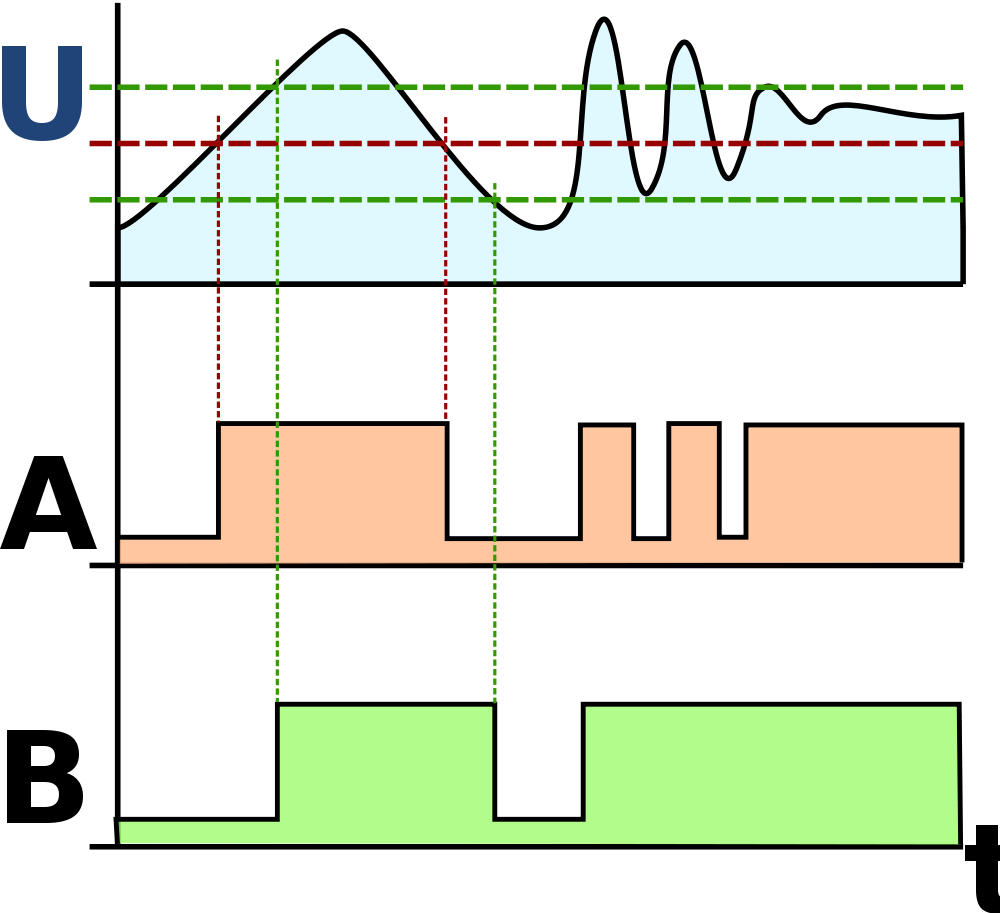
\includegraphics[height=7.5cm]{oskillaattori_pics/1000px-Smitt_hysteresis_graph.png}
%LÄHDE http://en.wikipedia.org/wiki/File:Smitt_hysteresis_graph.svg
\end{center}
}

\frame{
\frametitle{555-ajastinpiiri}
\begin{center}
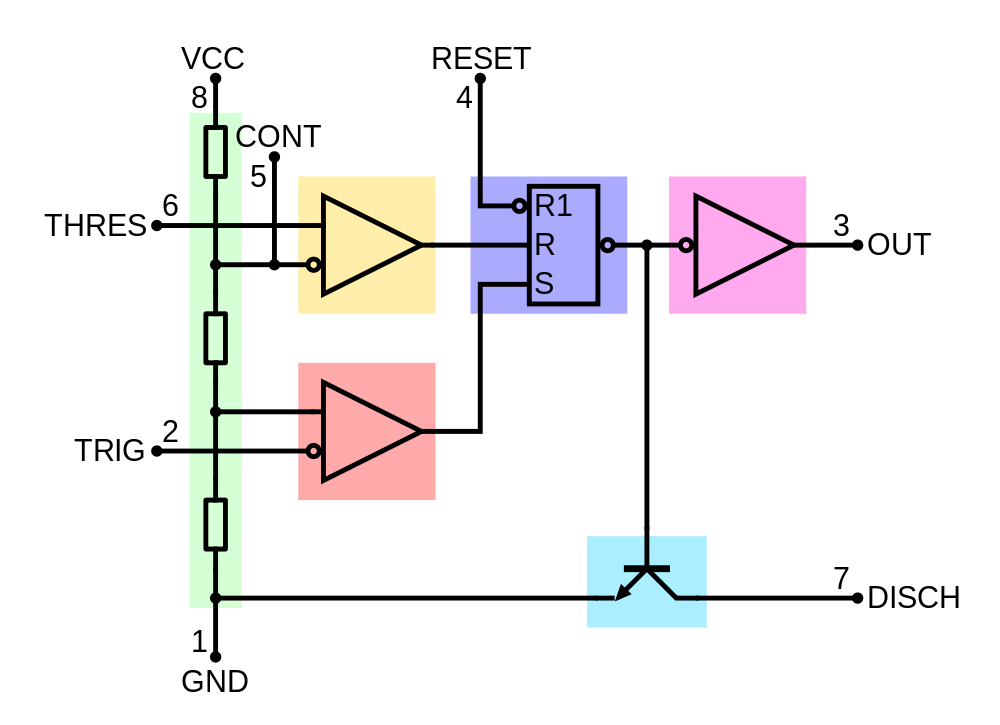
\includegraphics[height=6.5cm]{oskillaattori_pics/1000px-NE555_Bloc_Diagram.png}\\
%LÄHDE: http://en.wikipedia.org/wiki/File:NE555_Bloc_Diagram.svg
\end{center}
}



\frame {
\frametitle{Wienin siltaoskillaattori}

\begin{center}
\begin{picture}(150,200)(50,0)
\ho{50,125}{}
\hz{50,175}{}
\hz{0,175}{\rm PTC}
\hgp{0,175}

\hgp{100,0}
\vz{100,100}{R}
\vc{100,50}{C}

\vc{75,0}{C}
\vz{125,0}{R}
\hln{75,0}{50}
\hln{75,50}{50}

\hln{50,60}{50}
\vln{50,60}{65}

\vln{100,150}{25}
\cn{100,150}
\hln{100,150}{25}
\out{125,150}
\hgp{125,100}
\out{125,100}
\du{125,100}{\Uout}

\dcru{130,0}{U_+=\frac{1}{3+\jj(RC\omega-\frac{1}{RC\omega})}\Uout}

\end{picture}
\end{center}
 }

 \frame{
 \frametitle{Vaihesiirto-oskillaattori}
\begin{center}
\begin{picture}(250,120)(0,0)
\hc{0,50}{C}
\hc{50,50}{C}
\hc{100,50}{C}
\hz{150,50}{R}

\vz{50,0}{R}
\vz{100,0}{R}
\hg{50,0}
\hg{100,0}


\vo{200,30}{}{15}
\hgp{200,30}{}

\hz{200,90}{R_1}

\vln{200,50}{40}
\vln{250,40}{70}

\du{250,-10}{\Uout}
\hg{250,-10}

\hln{0,110}{250}
\vln{0,50}{60}

\end{picture}

\end{center}

 }

\frame{
\frametitle{Yhdenlainen relaksaatio-oskillaattori}

\begin{center}

\begin{picture}(110,130)(50,-50)

\hz{0,20}{R_1\ 1\kohm}
\voi{50,0}{}{15}
\hz{50,60}{R_2\ 15\kohm}
\hgp{50,0}

\hz{100,10}{R_3\ 150 \kohm}
\vo{150,-10}{}{15}
\hgp{150,-10}
\hc{150,50}{C\ 100\ \mbox{nF}}

\vln{200,0}{75}
\hln{100,75}{100}
\vln{150,10}{40}
\vln{0,20}{55}
\hln{0,75}{100}

\vln{50,20}{40}
\vln{100,10}{50}

\hln{200,0}{10}
\du{210,-50}{\Uout}
\hg{210,-50}

\end{picture}
\end{center}

Vasemmalla puolella on Schmitt-liipaisintulolla varustettu komparaattori ja oikealla puolella on integraattori. Yhdessä piirit muodostavat kokonaisuuden, jossa kondensaattori latautuu ja purkautuu jatkuvasti.

}
